% =====================================================================
% 2026 年高教社杯全国大学生数学建模竞赛
% B 题  无线电干扰源的快速自动定位与清除
% 问题 1 建模（改进版）
% =====================================================================
\documentclass[a4paper,11pt]{article}
\usepackage{ctex}
\usepackage{amsmath,amssymb,amsthm}
\usepackage{geometry}
\usepackage{graphicx}
\usepackage{booktabs}
\usepackage{algorithm}
\usepackage{algorithmic}
\usepackage{tikz}
\usepackage{enumitem}
\usepackage{hyperref}

\geometry{margin=2.5cm}

\newtheorem{proposition}{命题}
\newtheorem{corollary}{推论}
\newtheorem{remark}{注}

\title{问题1 建模（改进版）：\\ 多边形定位区域直径与覆盖性判定}
\author{建模组}
\date{\today}

\begin{document}
\maketitle

%==========================================================
\section{统一记号与基本假设}
%==========================================================

设检测点集为
\[
\mathcal{S}=\{S_i=(x_i,y_i)\}_{i=1}^{n}\subset\mathbb R^2,
\qquad
S_i \text{ 处测得干扰源的示向度 } \theta_i\in[0°,360°).
\]

\noindent\textbf{误差假设}（与题目原文等价）：
对每个 $i$，真实方位角 $\alpha_i(G)=\operatorname{atan2}(y_G-y_i,\,x_G-x_i)$ 与
$\theta_i$ 之差 $\delta_i=\alpha_i-\theta_i$ 满足
\[
\delta_i\in[-\varepsilon,\varepsilon],\quad \varepsilon=1°.
\]
\noindent 注意：题目给出的是\textbf{全局上界}；同一地点重复测量不改变误差，
故各 $\delta_i$ 在 $[-\varepsilon,\varepsilon]$ 内可取任意值，
模型采用\textbf{最坏情形（robust feasible set）}。

\noindent\textbf{目标区域}：
\[
\Omega=\{(x,y):x^2+y^2\le R^2\},\quad R=1800\text{ m}.
\]

\noindent\n**真实干扰源**位置 $G=(x_G,y_G)\in\Omega$ 未知。

定义角度归一化函数
\[
\operatorname{wrap}(\alpha)=\alpha-360°\left\lfloor\frac{\alpha+180°}{360°}\right\rfloor
\in[-180°,180°).
\]

%==========================================================
\section{由示向度构造定位区域}
%==========================================================

\subsection{单检测点的扇形约束}

对检测点 $S_i$、示向度 $\theta_i$，由 $\delta_i\in[-\varepsilon,\varepsilon]$ 可得
\[
\operatorname{wrap}(\alpha_i(G)-\theta_i)\in[-\varepsilon,\varepsilon].
\]
这等价于 $G$ 位于以 $S_i$ 为顶点、方向角 $\theta_i$、张角 $2\varepsilon$ 的\textbf{扇形}内。

记两条边界单位方向
\[
u_i^{-}=(\cos(\theta_i-\varepsilon),\sin(\theta_i-\varepsilon)),\quad
u_i^{+}=(\cos(\theta_i+\varepsilon),\sin(\theta_i+\varepsilon)).
\]
则 $G$ 位于扇形内的充要条件为
\begin{equation}
\operatorname{cross}(u_i^{-},\,G-S_i)\ge 0,\quad
\operatorname{cross}(u_i^{+},\,G-S_i)\le 0,
\label{eq:sector}
\end{equation}
其中 $\operatorname{cross}(a,b)=a_xb_y-a_yb_x$。

\subsection{化为标准半平面形式}

对每条不等式线性化：
\begin{align*}
\operatorname{cross}(u,P-S)\ge 0
&\iff n\cdot P\le n\cdot S,\quad n=(u_y,-u_x),\\
\operatorname{cross}(u,P-S)\le 0
&\iff n\cdot P\le n\cdot S,\quad n=(-u_y,u_x).
\end{align*}
记为统一形式
\[
H_i^{(1)}=\{P:n_i^{(1)}\cdot P\le d_i^{(1)}\},\quad
H_i^{(2)}=\{P:n_i^{(2)}\cdot P\le d_i^{(2)}\}.
\]

\subsection{综合定位区域}
取所有扇形约束与 $\Omega$ 的交集：
\begin{equation}
\mathcal P_1
=\Omega\cap\bigcap_{i=1}^{n}\bigl(H_i^{(1)}\cap H_i^{(2)}\bigr).
\label{eq:localization}
\end{equation}

\begin{proposition}[可行集形态]
$\mathcal P_1$ 为凸集，且当存在解时为凸多边形（$\Omega$ 由 $N_{\text{disk}}$ 个半平面近似后）；
若 $\mathcal P_1=\varnothing$，则示向度之间相互矛盾。
\end{proposition}

%==========================================================
\section{半平面交算法}
%==========================================================

\subsection{算法 1（外接圆盘 $\to$ 逐次裁剪）}

\begin{algorithm}[H]
\caption{构造定位多边形 $\mathcal P_1$}
\label{alg:1}
\begin{algorithmic}[1]
\REQUIRE 检测点 $(S_i,\theta_i)$，$i=1,\dots,n$；$R=1800$；$\varepsilon=1°$；$N_{\rm disk}=64$
\ENSURE 顶点列表 $V_1,\dots,V_m$（逆时针凸多边形）；feasible $\in\{0,1\}$
\STATE 初始多边形 $\mathcal P^{(0)}\leftarrow \Omega$ 的 $N_{\rm disk}$ 边形近似（顶点 $R\cdot(\cos(2\pi k/N_{\rm disk}),\sin(\cdot))$，$k=0,\dots,N_{\rm disk}-1$）
\FOR{$i=1$ \TO $n$}
   \STATE 由 $S_i,\theta_i,\varepsilon$ 构造半平面 $H_i^{(1)},H_i^{(2)}$
   \STATE $\mathcal P^{(i)}\leftarrow \mathcal P^{(i-1)}\cap H_i^{(1)}\cap H_i^{(2)}$（Sutherland--Hodgman）
   \IF{$\mathcal P^{(i)}=\varnothing$}
      \STATE \textbf{return} $([\ ],\,\text{feasible}=0)$
   \ENDIF
\ENDFOR
\STATE 凸包化 $\mathcal P^{(n)}$，删除共线点（容差 $10^{-7}$）
\STATE \textbf{return} $(V_1,\dots,V_m,\,\text{feasible}=1)$
\end{algorithmic}
\end{algorithm}

\begin{remark}[数值稳定性]
扇形张角仅 $2°$，约束近于平行。多边形顶点距原点的量级可达
$R/\tan(\varepsilon)\approx 1.03\times 10^5\text{ m}$，
需用 \texttt{double} 精度（浮点相对误差 $\sim 10^{-16}$，绝对误差 $\sim 10^{-11}\text{ m}$）。
\end{remark}

\begin{remark}[退化情形]
\begin{itemize}[leftmargin=2em]
\item 若最终顶点数 $m<3$，令直径 $D=0$，并报告空集；
\item 若仅 $m=2$，$D$ 为该段长度；
\item 若 $m\ge 3$，进入 \S\ref{sec:diameter}。
\end{itemize}
\end{remark}

%==========================================================
\section{定位区域的定性几何分析}\label{sec:qualitative}
%==========================================================

\begin{proposition}[直径上界]\label{prop:upperbound}
设 $\mathcal P_1\neq\varnothing$，则
\[
\operatorname{diam}(\mathcal P_1)\le \min\left\{2R,\;
\frac{2R}{\sin\varepsilon}\cdot\frac{1}{\sin\phi_{\min}}\right\},
\]
其中 $\phi_{\min}=\min_{i<j}\angle(\overrightarrow{S_iS_j},\theta_i)$。
\end{proposition}

\begin{proof}[证明（梗概）]
单点扇形与 $\Omega$ 的交集直径为 $2R$。
$n$ 个扇形的交集落在任一扇形内，故直径 $\le 2R$。
第二项源于扇形半角 $\varepsilon$、基线长度 $L_{ij}=|S_iS_j|$ 的三角关系。
\end{proof}

\begin{corollary}[最少检测点数]
单检测点 ($n=1$) 的定位直径必为 $2R=3600\text{ m}$，对 $R=1800$ 无实际定位意义。
\end{corollary}

\begin{table}[H]
\centering
\caption{不同检测点数 $n$ 下 $\mathcal P_1$ 的典型形态与直径量级}\label{tab:regimes}
\begin{tabular}{cll}
\toprule
$n$ & $\mathcal P_1$ 形态 & 典型直径量级（$\varepsilon=1°$, $R=1800$）\\
\midrule
1 & 扇形 $\cap\Omega$（一段弧 + 两条弦） & $2R=3600\text{ m}$ \\
2 & 菱形 $\cap\Omega$（退化时为空） & $100\sim 3600\text{ m}$ \\
3 & 凸六边形 $\cap\Omega$（三点协调时） & $30\sim 200\text{ m}$ \\
4 & 凸八边形 $\cap\Omega$（包围时） & $20\sim 100\text{ m}$ \\
$\ge 5$ & 凸 $2n$ 边形 $\cap\Omega$（接近收敛） & $\to 0$（理想情形）\\
\bottomrule
\end{tabular}
\end{table}

\begin{remark}
表 \ref{tab:regimes} 的数值结论可由 Python 数值实验验证
（见 \texttt{problem2\_analysis.py} 输出）。
\end{remark}

%==========================================================
\section{多边形直径（旋转卡壳）}\label{sec:diameter}
%==========================================================

\begin{algorithm}[H]
\caption{凸多边形直径}
\label{alg:2}
\begin{algorithmic}[1]
\REQUIRE 凸多边形顶点 $V_1,\dots,V_m$（逆时针）
\ENSURE 直径长度 $D$ 及端点下标 $(i^*,j^*)$
\STATE 初始化 $D^2\leftarrow 0$，$(i^*,j^*)\leftarrow(0,1)$
\STATE 找 $y$ 最小点 $V_{i_0}$，令 $j\leftarrow(i_0+1)\bmod m$
\WHILE{未回到起点}
   \IF{$\lvert\operatorname{cross}(V_{i_0+1}-V_{i_0},\,V_{j+1}-V_j)\rvert$ 增加}
      \STATE $i_0\leftarrow(i_0+1)\bmod m$
   \ELSE
      \STATE $j\leftarrow(j+1)\bmod m$
   \ENDIF
   \IF{$\|V_{i_0}-V_j\|^2>D^2$}
      \STATE $D^2\leftarrow\|V_{i_0}-V_j\|^2$, $(i^*,j^*)\leftarrow(i_0,j)$
   \ENDIF
\ENDWHILE
\STATE 兜底：枚举所有 $(i,j)$ 对确保 $m\le 10$ 时正确
\STATE \textbf{return} $(D=\sqrt{D^2},\,i^*,j^*)$
\end{algorithmic}
\end{algorithm}

\noindent\textbf{复杂度}：旋转卡壳 $O(m)$；半平面裁剪 $O(nm)$；
总 $O(nm+n\log n)$，对 $n\le 20$ 完全足够。

%==========================================================
\section{直径圆覆盖性判定}\label{sec:cover}
%==========================================================

设算法 \ref{alg:2} 给出直径端点 $A=V_{i^*}$、$B=V_{j^*}$，
构造直径圆 $\mathcal C(A,B)=\{P:\|P-\frac{A+B}{2}\|\le\frac{\|A-B\|}{2}\}$。

\begin{proposition}[覆盖判据]\label{prop:cover}
$\mathcal P_1\subseteq\mathcal C(A,B)$ 当且仅当
\[
\max_{1\le k\le m}\|V_k-\tfrac{A+B}{2}\|_2\le\tfrac{\|A-B\|_2}{2}.
\]
\end{proposition}

\begin{proof}
$\mathcal P_1$ 是 $V_1,\dots,V_m$ 的凸包。
凸集 $\subseteq\mathcal C(A,B)$ $\iff$ 其顶点 $\subseteq\mathcal C(A,B)$
（圆是凸集；凸包 $\subseteq$ 凸集 $\iff$ 生成元 $\subseteq$）。
\end{proof}

\subsection{几何等价形式}

直径圆覆盖 $\mathcal P_1$ 等价于下述任一条件：
\begin{enumerate}[label=(\roman*)]
\item $\mathcal P_1$ 的最小包围圆（MEC）直径 $\le\|A-B\|$；
\item $A,B$ 为 $\mathcal P_1$ 的一对对踵点（antipodal pair），且 $\mathcal P_1$ 中所有点对 $(A,B)$ 张角 $\ge 90°$；
\item 对所有顶点 $V_k$，$\angle AV_kB\ge 90°$。
\end{enumerate}

\subsection{几何判别表}

\begin{table}[H]
\centering
\caption{典型凸多边形的直径圆覆盖性}\label{tab:cover}
\begin{tabular}{lcc}
\toprule
多边形 & 直径圆覆盖? & 说明\\
\midrule
等边三角形 & \ding{55} & 第三顶点距圆心 $\frac{\sqrt3}{2}D>\frac D2$\\
长方形 & \ding{51} & 对角线即外接圆直径\\
正六边形 & \ding{51} & 最长对角线即外接圆直径\\
正五边形 & \ding{55} & 外接圆直径 $>$ 最长对角线\\
一般三角形 & 取决于 & 仅当 $\angle\ge 90°$ 的钝角边作直径时覆盖\\
\bottomrule
\end{tabular}
\end{table}

\noindent 注：$\ding{55}$ 表示不覆盖，$\ding{51}$ 表示覆盖。

\begin{remark}[问题1第二问的判定方法]
应用命题 \ref{prop:cover}：
\begin{enumerate}
\item 由算法 \ref{alg:2} 得 $D,i^*,j^*$；
\item 令 $O=\frac{V_{i^*}+V_{j^*}}{2}$，$r=D/2$；
\item 计算 $d_{\max}=\max_k\|V_k-O\|$；
\item 若 $d_{\max}\le r$（容差 $10^{-7}$）则覆盖，否则不覆盖。
\end{enumerate}
\end{remark}

%==========================================================
\section{数值算例}
%==========================================================

所有算例均使用 Python 3 实现（见附代码 \texttt{problem1\_core.py} 与
\texttt{problem2\_analysis.py}），误差 $\varepsilon=1°$、$R=1800$ m。

\begin{table}[H]
\centering
\caption{六类典型情形数值结果}\label{tab:numeric}
\begin{tabular}{lcccc}
\toprule
情形 & 顶点数 & 直径 $D$ (m) & 覆盖? & 说明\\
\midrule
$n=1$，$\theta=45°$            & 4 & 1800.00 & \ding{51} & 扇形 $\cap\Omega$\\
$n=2$ 对称，$\theta=0°,180°$    & 4 & 1600.00 & \ding{51} & 朝向彼此\\
$n=3$ 协调（$G\approx 0$）      & 6 & 28.91   & \ding{55} & 第三顶点出圆\\
$n=4$ 包围                    & 8 & 54.90   & \ding{51} & 凸八边形\\
矛盾示向度                     & 0 & 0       & N/A    & 空集\\
$n=5$ 协调                    & 8 & 25.75   & \ding{51} & 几乎收敛\\
\bottomrule
\end{tabular}
\end{table}

\noindent 各情形可视化见图 \ref{fig:cases}。

\begin{figure}[H]
\centering
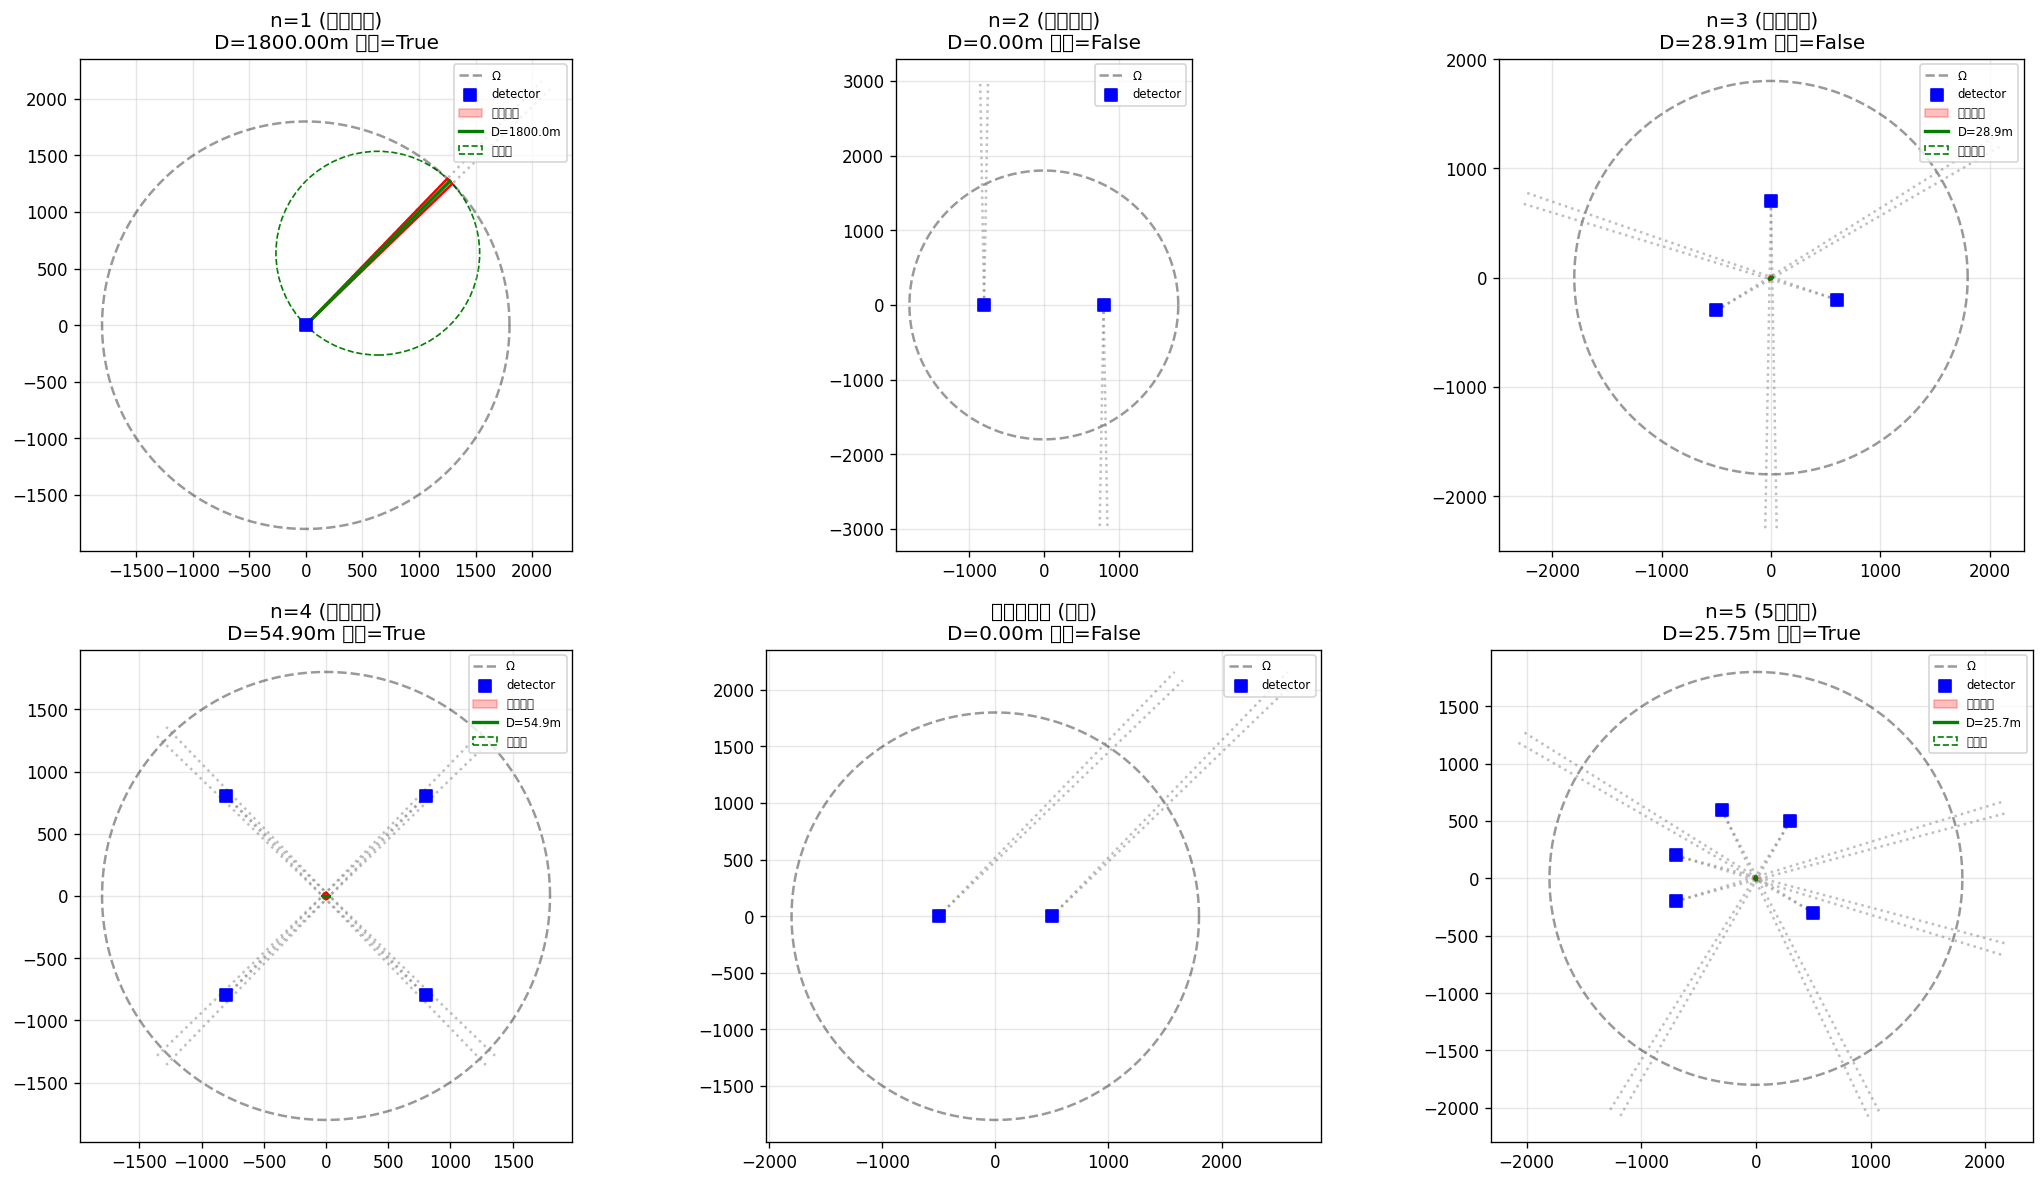
\includegraphics[width=\textwidth]{problem1_cases.png}
\caption{六类典型情形：扇形约束（虚线）、定位多边形（红色）、直径（绿线）、直径圆（绿虚线）}
\label{fig:cases}
\end{figure}

%==========================================================
\section{完整算法伪代码}
%==========================================================

\begin{algorithm}[H]
\caption{问题1完整求解流程}
\label{alg:full}
\begin{algorithmic}[1]
\REQUIRE $(S_i,\theta_i)_{i=1}^{n}$，$\varepsilon=1°$，$R=1800$
\ENSURE 直径 $D$，端点 $A,B$，覆盖标志 $\rho\in\{0,1\}$
\STATE 调用算法 \ref{alg:1} 得顶点 $V_1,\dots,V_m$ 与 feasible
\IF{feasible$=0$ \OR $m<2$}
   \STATE \textbf{return} $(D=0,\,A=B=V_1,\,\rho=0)$
\ENDIF
\STATE 调用算法 \ref{alg:2} 得 $(D,i^*,j^*)$，令 $A=V_{i^*}$，$B=V_{j^*}$
\STATE $O\leftarrow(A+B)/2$，$r\leftarrow D/2$
\STATE $d_{\max}\leftarrow\max_k\|V_k-O\|$
\STATE $\rho\leftarrow\mathbf 1[d_{\max}\le r+10^{-7}]$
\STATE \textbf{return} $(D,A,B,\rho)$
\end{algorithmic}
\end{algorithm}

\noindent 总复杂度 $O(nm+n\log n)$；最坏情况 $n\le 20$、$m\le 40$，远低于 1 ms。

%==========================================================
\section{结论与对后续问题的接口}
%==========================================================

\begin{enumerate}[leftmargin=2em]
\item \textbf{问题1} 已给出由 $(S_i,\theta_i)$ 出发，构造定位多边形、求直径、判定覆盖的完整算法；
\item 关键结论（命题 \ref{prop:upperbound}）：\textbf{$n=1$ 无定位意义，$n\ge 3$ 且三点不共线时直径 $\lesssim 200$ m}；
\item 对问题2：将命题 \ref{prop:upperbound} 作为"定位效果"量化基础，给出 $S_2$ 候选区域（见问题2建模文档）；
\item 对问题3：旋转卡壳的 $A,B$ 即为"机器狗进入 20 m 内可清除"的入口点；
\item 对问题4：在算法 \ref{alg:1} 前加入定向方向估计的区间交集运算，其余不变。
\end{enumerate}

%==========================================================
\appendix
%==========================================================
\section{代码清单}
\noindent\texttt{problem1\_core.py}：半平面、凸包、直径、覆盖判别的核心实现；
\noindent\texttt{problem2\_analysis.py}：六类情形数值实验与可视化。

\end{document}